% Created by tikzDevice version 0.12 on 2018-08-21 16:29:48
% !TEX encoding = UTF-8 Unicode
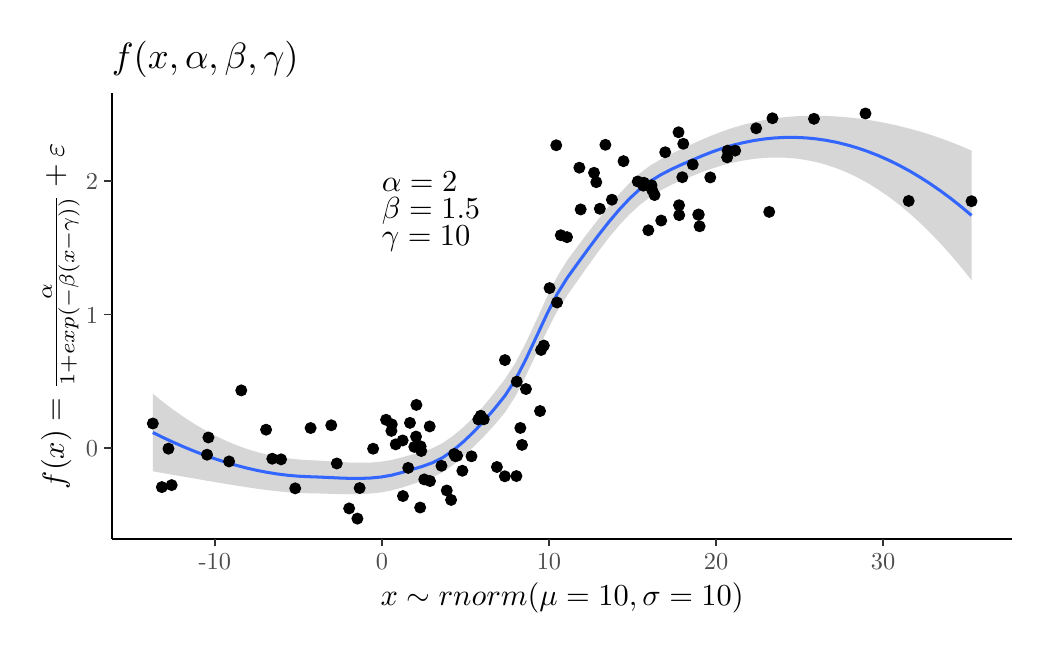
\begin{tikzpicture}[x=1pt,y=1pt]
\definecolor{fillColor}{RGB}{255,255,255}
\path[use as bounding box,fill=fillColor,fill opacity=0.00] (0,0) rectangle (361.35,216.81);
\begin{scope}
\path[clip] (  0.00,  0.00) rectangle (361.35,216.81);
\definecolor{drawColor}{RGB}{255,255,255}
\definecolor{fillColor}{RGB}{255,255,255}

\path[draw=drawColor,line width= 0.6pt,line join=round,line cap=round,fill=fillColor] (  0.00,  0.00) rectangle (361.35,216.81);
\end{scope}
\begin{scope}
\path[clip] ( 30.42, 32.09) rectangle (355.85,193.12);
\definecolor{fillColor}{RGB}{255,255,255}

\path[fill=fillColor] ( 30.42, 32.09) rectangle (355.85,193.12);
\definecolor{fillColor}{RGB}{153,153,153}

\path[fill=fillColor,fill opacity=0.40] ( 45.22, 84.54) --
	( 48.96, 81.53) --
	( 52.71, 78.70) --
	( 56.45, 76.08) --
	( 60.20, 73.65) --
	( 63.94, 71.43) --
	( 67.69, 69.42) --
	( 71.43, 67.63) --
	( 75.18, 66.04) --
	( 78.92, 64.67) --
	( 82.66, 63.51) --
	( 86.41, 62.55) --
	( 90.15, 61.78) --
	( 93.90, 61.20) --
	( 97.64, 60.79) --
	(101.39, 60.54) --
	(105.13, 60.37) --
	(108.88, 60.14) --
	(112.62, 59.89) --
	(116.37, 59.68) --
	(120.11, 59.59) --
	(123.86, 59.66) --
	(127.60, 59.97) --
	(131.35, 60.56) --
	(135.09, 61.48) --
	(138.84, 62.53) --
	(142.58, 63.54) --
	(146.33, 64.86) --
	(150.07, 66.78) --
	(153.82, 69.40) --
	(157.56, 72.53) --
	(161.31, 76.21) --
	(165.05, 80.44) --
	(168.80, 85.08) --
	(172.54, 89.94) --
	(176.29, 95.75) --
	(180.03,102.97) --
	(183.78,111.01) --
	(187.52,119.19) --
	(191.26,126.73) --
	(195.01,132.79) --
	(198.75,137.85) --
	(202.50,142.80) --
	(206.24,147.61) --
	(209.99,152.26) --
	(213.73,156.66) --
	(217.48,160.69) --
	(221.22,164.19) --
	(224.97,166.99) --
	(228.71,169.23) --
	(232.46,171.17) --
	(236.20,172.95) --
	(239.95,174.66) --
	(243.69,176.37) --
	(247.44,177.96) --
	(251.18,179.38) --
	(254.93,180.65) --
	(258.67,181.74) --
	(262.42,182.66) --
	(266.16,183.42) --
	(269.91,184.03) --
	(273.65,184.48) --
	(277.40,184.79) --
	(281.14,184.96) --
	(284.89,185.00) --
	(288.63,184.92) --
	(292.38,184.73) --
	(296.12,184.42) --
	(299.86,184.01) --
	(303.61,183.49) --
	(307.35,182.86) --
	(311.10,182.13) --
	(314.84,181.30) --
	(318.59,180.36) --
	(322.33,179.31) --
	(326.08,178.15) --
	(329.82,176.88) --
	(333.57,175.50) --
	(337.31,174.00) --
	(341.06,172.39) --
	(341.06,125.55) --
	(337.31,130.24) --
	(333.57,134.67) --
	(329.82,138.84) --
	(326.08,142.75) --
	(322.33,146.40) --
	(318.59,149.78) --
	(314.84,152.89) --
	(311.10,155.74) --
	(307.35,158.32) --
	(303.61,160.63) --
	(299.86,162.68) --
	(296.12,164.46) --
	(292.38,165.98) --
	(288.63,167.25) --
	(284.89,168.25) --
	(281.14,169.02) --
	(277.40,169.54) --
	(273.65,169.83) --
	(269.91,169.89) --
	(266.16,169.74) --
	(262.42,169.39) --
	(258.67,168.83) --
	(254.93,168.07) --
	(251.18,167.11) --
	(247.44,165.96) --
	(243.69,164.61) --
	(239.95,163.12) --
	(236.20,161.62) --
	(232.46,159.95) --
	(228.71,157.99) --
	(224.97,155.63) --
	(221.22,152.78) --
	(217.48,149.35) --
	(213.73,145.37) --
	(209.99,140.89) --
	(206.24,135.98) --
	(202.50,130.78) --
	(198.75,125.44) --
	(195.01,120.15) --
	(191.26,114.20) --
	(187.52,106.96) --
	(183.78, 99.01) --
	(180.03, 91.00) --
	(176.29, 83.68) --
	(172.54, 77.87) --
	(168.80, 73.39) --
	(165.05, 69.32) --
	(161.31, 65.54) --
	(157.56, 62.02) --
	(153.82, 58.86) --
	(150.07, 56.24) --
	(146.33, 54.37) --
	(142.58, 52.99) --
	(138.84, 51.79) --
	(135.09, 50.58) --
	(131.35, 49.57) --
	(127.60, 48.88) --
	(123.86, 48.47) --
	(120.11, 48.26) --
	(116.37, 48.21) --
	(112.62, 48.27) --
	(108.88, 48.38) --
	(105.13, 48.50) --
	(101.39, 48.57) --
	( 97.64, 48.71) --
	( 93.90, 48.96) --
	( 90.15, 49.32) --
	( 86.41, 49.75) --
	( 82.66, 50.25) --
	( 78.92, 50.79) --
	( 75.18, 51.38) --
	( 71.43, 51.99) --
	( 67.69, 52.61) --
	( 63.94, 53.25) --
	( 60.20, 53.90) --
	( 56.45, 54.55) --
	( 52.71, 55.20) --
	( 48.96, 55.86) --
	( 45.22, 56.51) --
	cycle;
\definecolor{drawColor}{RGB}{51,102,255}

\path[draw=drawColor,line width= 1.1pt,line join=round] ( 45.22, 70.53) --
	( 48.96, 68.69) --
	( 52.71, 66.95) --
	( 56.45, 65.31) --
	( 60.20, 63.77) --
	( 63.94, 62.34) --
	( 67.69, 61.02) --
	( 71.43, 59.81) --
	( 75.18, 58.71) --
	( 78.92, 57.73) --
	( 82.66, 56.88) --
	( 86.41, 56.15) --
	( 90.15, 55.55) --
	( 93.90, 55.08) --
	( 97.64, 54.75) --
	(101.39, 54.56) --
	(105.13, 54.43) --
	(108.88, 54.26) --
	(112.62, 54.08) --
	(116.37, 53.95) --
	(120.11, 53.93) --
	(123.86, 54.07) --
	(127.60, 54.43) --
	(131.35, 55.06) --
	(135.09, 56.03) --
	(138.84, 57.16) --
	(142.58, 58.26) --
	(146.33, 59.61) --
	(150.07, 61.51) --
	(153.82, 64.13) --
	(157.56, 67.28) --
	(161.31, 70.88) --
	(165.05, 74.88) --
	(168.80, 79.23) --
	(172.54, 83.90) --
	(176.29, 89.71) --
	(180.03, 96.99) --
	(183.78,105.01) --
	(187.52,113.07) --
	(191.26,120.46) --
	(195.01,126.47) --
	(198.75,131.65) --
	(202.50,136.79) --
	(206.24,141.80) --
	(209.99,146.58) --
	(213.73,151.02) --
	(217.48,155.02) --
	(221.22,158.49) --
	(224.97,161.31) --
	(228.71,163.61) --
	(232.46,165.56) --
	(236.20,167.29) --
	(239.95,168.89) --
	(243.69,170.49) --
	(247.44,171.96) --
	(251.18,173.25) --
	(254.93,174.36) --
	(258.67,175.28) --
	(262.42,176.02) --
	(266.16,176.58) --
	(269.91,176.96) --
	(273.65,177.15) --
	(277.40,177.16) --
	(281.14,176.99) --
	(284.89,176.63) --
	(288.63,176.08) --
	(292.38,175.36) --
	(296.12,174.44) --
	(299.86,173.34) --
	(303.61,172.06) --
	(307.35,170.59) --
	(311.10,168.94) --
	(314.84,167.10) --
	(318.59,165.07) --
	(322.33,162.85) --
	(326.08,160.45) --
	(329.82,157.86) --
	(333.57,155.09) --
	(337.31,152.12) --
	(341.06,148.97);
\definecolor{drawColor}{RGB}{0,0,0}
\definecolor{fillColor}{RGB}{0,0,0}

\path[draw=drawColor,line width= 0.4pt,line join=round,line cap=round,fill=fillColor] (188.59,122.71) circle (  1.96);

\path[draw=drawColor,line width= 0.4pt,line join=round,line cap=round,fill=fillColor] (236.55,162.77) circle (  1.96);

\path[draw=drawColor,line width= 0.4pt,line join=round,line cap=round,fill=fillColor] (242.30,149.24) circle (  1.96);

\path[draw=drawColor,line width= 0.4pt,line join=round,line cap=round,fill=fillColor] (116.17, 43.09) circle (  1.96);

\path[draw=drawColor,line width= 0.4pt,line join=round,line cap=round,fill=fillColor] (111.70, 59.33) circle (  1.96);

\path[draw=drawColor,line width= 0.4pt,line join=round,line cap=round,fill=fillColor] (199.35,166.21) circle (  1.96);

\path[draw=drawColor,line width= 0.4pt,line join=round,line cap=round,fill=fillColor] (109.70, 73.13) circle (  1.96);

\path[draw=drawColor,line width= 0.4pt,line join=round,line cap=round,fill=fillColor] (176.60, 54.78) circle (  1.96);

\path[draw=drawColor,line width= 0.4pt,line join=round,line cap=round,fill=fillColor] (263.25,180.44) circle (  1.96);

\path[draw=drawColor,line width= 0.4pt,line join=round,line cap=round,fill=fillColor] (240.33,167.37) circle (  1.96);

\path[draw=drawColor,line width= 0.4pt,line join=round,line cap=round,fill=fillColor] (220.44,161.24) circle (  1.96);

\path[draw=drawColor,line width= 0.4pt,line join=round,line cap=round,fill=fillColor] (138.14, 74.01) circle (  1.96);

\path[draw=drawColor,line width= 0.4pt,line join=round,line cap=round,fill=fillColor] ( 91.56, 60.82) circle (  1.96);

\path[draw=drawColor,line width= 0.4pt,line join=round,line cap=round,fill=fillColor] (252.94,172.38) circle (  1.96);

\path[draw=drawColor,line width= 0.4pt,line join=round,line cap=round,fill=fillColor] (129.51, 75.12) circle (  1.96);

\path[draw=drawColor,line width= 0.4pt,line join=round,line cap=round,fill=fillColor] ( 96.67, 50.34) circle (  1.96);

\path[draw=drawColor,line width= 0.4pt,line join=round,line cap=round,fill=fillColor] (137.50, 57.74) circle (  1.96);

\path[draw=drawColor,line width= 0.4pt,line join=round,line cap=round,fill=fillColor] (149.52, 58.49) circle (  1.96);

\path[draw=drawColor,line width= 0.4pt,line join=round,line cap=round,fill=fillColor] (140.47, 80.49) circle (  1.96);

\path[draw=drawColor,line width= 0.4pt,line join=round,line cap=round,fill=fillColor] ( 65.31, 68.73) circle (  1.96);

\path[draw=drawColor,line width= 0.4pt,line join=round,line cap=round,fill=fillColor] (236.90,174.85) circle (  1.96);

\path[draw=drawColor,line width= 0.4pt,line join=round,line cap=round,fill=fillColor] ( 45.22, 73.78) circle (  1.96);

\path[draw=drawColor,line width= 0.4pt,line join=round,line cap=round,fill=fillColor] (225.43,159.86) circle (  1.96);

\path[draw=drawColor,line width= 0.4pt,line join=round,line cap=round,fill=fillColor] (102.24, 72.14) circle (  1.96);

\path[draw=drawColor,line width= 0.4pt,line join=round,line cap=round,fill=fillColor] (154.11, 62.75) circle (  1.96);

\path[draw=drawColor,line width= 0.4pt,line join=round,line cap=round,fill=fillColor] (255.65,172.38) circle (  1.96);

\path[draw=drawColor,line width= 0.4pt,line join=round,line cap=round,fill=fillColor] ( 72.78, 60.07) circle (  1.96);

\path[draw=drawColor,line width= 0.4pt,line join=round,line cap=round,fill=fillColor] (162.84, 75.24) circle (  1.96);

\path[draw=drawColor,line width= 0.4pt,line join=round,line cap=round,fill=fillColor] (206.74,151.37) circle (  1.96);

\path[draw=drawColor,line width= 0.4pt,line join=round,line cap=round,fill=fillColor] (151.44, 49.57) circle (  1.96);

\path[draw=drawColor,line width= 0.4pt,line join=round,line cap=round,fill=fillColor] (163.70, 76.59) circle (  1.96);

\path[draw=drawColor,line width= 0.4pt,line join=round,line cap=round,fill=fillColor] (178.03, 72.17) circle (  1.96);

\path[draw=drawColor,line width= 0.4pt,line join=round,line cap=round,fill=fillColor] (228.93,147.11) circle (  1.96);

\path[draw=drawColor,line width= 0.4pt,line join=round,line cap=round,fill=fillColor] ( 48.49, 50.79) circle (  1.96);

\path[draw=drawColor,line width= 0.4pt,line join=round,line cap=round,fill=fillColor] (192.64,141.81) circle (  1.96);

\path[draw=drawColor,line width= 0.4pt,line join=round,line cap=round,fill=fillColor] (242.51,149.27) circle (  1.96);

\path[draw=drawColor,line width= 0.4pt,line join=round,line cap=round,fill=fillColor] (191.29,117.51) circle (  1.96);

\path[draw=drawColor,line width= 0.4pt,line join=round,line cap=round,fill=fillColor] (222.67,160.77) circle (  1.96);

\path[draw=drawColor,line width= 0.4pt,line join=round,line cap=round,fill=fillColor] (141.83, 43.41) circle (  1.96);

\path[draw=drawColor,line width= 0.4pt,line join=round,line cap=round,fill=fillColor] ( 86.15, 71.54) circle (  1.96);

\path[draw=drawColor,line width= 0.4pt,line join=round,line cap=round,fill=fillColor] (139.71, 65.33) circle (  1.96);

\path[draw=drawColor,line width= 0.4pt,line join=round,line cap=round,fill=fillColor] (267.95,150.24) circle (  1.96);

\path[draw=drawColor,line width= 0.4pt,line join=round,line cap=round,fill=fillColor] (318.35,154.20) circle (  1.96);

\path[draw=drawColor,line width= 0.4pt,line join=round,line cap=round,fill=fillColor] (252.76,169.95) circle (  1.96);

\path[draw=drawColor,line width= 0.4pt,line join=round,line cap=round,fill=fillColor] (341.06,154.10) circle (  1.96);

\path[draw=drawColor,line width= 0.4pt,line join=round,line cap=round,fill=fillColor] (204.66,164.36) circle (  1.96);

\path[draw=drawColor,line width= 0.4pt,line join=round,line cap=round,fill=fillColor] (235.19,179.01) circle (  1.96);

\path[draw=drawColor,line width= 0.4pt,line join=round,line cap=round,fill=fillColor] (211.11,154.65) circle (  1.96);

\path[draw=drawColor,line width= 0.4pt,line join=round,line cap=round,fill=fillColor] ( 88.39, 61.05) circle (  1.96);

\path[draw=drawColor,line width= 0.4pt,line join=round,line cap=round,fill=fillColor] (145.38, 52.98) circle (  1.96);

\path[draw=drawColor,line width= 0.4pt,line join=round,line cap=round,fill=fillColor] (160.37, 61.92) circle (  1.96);

\path[draw=drawColor,line width= 0.4pt,line join=round,line cap=round,fill=fillColor] (145.27, 72.72) circle (  1.96);

\path[draw=drawColor,line width= 0.4pt,line join=round,line cap=round,fill=fillColor] (169.56, 58.06) circle (  1.96);

\path[draw=drawColor,line width= 0.4pt,line join=round,line cap=round,fill=fillColor] (176.74, 88.90) circle (  1.96);

\path[draw=drawColor,line width= 0.4pt,line join=round,line cap=round,fill=fillColor] ( 52.03, 51.51) circle (  1.96);

\path[draw=drawColor,line width= 0.4pt,line join=round,line cap=round,fill=fillColor] (235.43,149.06) circle (  1.96);

\path[draw=drawColor,line width= 0.4pt,line join=round,line cap=round,fill=fillColor] (185.52,100.35) circle (  1.96);

\path[draw=drawColor,line width= 0.4pt,line join=round,line cap=round,fill=fillColor] (242.80,145.04) circle (  1.96);

\path[draw=drawColor,line width= 0.4pt,line join=round,line cap=round,fill=fillColor] (172.46, 96.69) circle (  1.96);

\path[draw=drawColor,line width= 0.4pt,line join=round,line cap=round,fill=fillColor] (154.54, 61.98) circle (  1.96);

\path[draw=drawColor,line width= 0.4pt,line join=round,line cap=round,fill=fillColor] (140.34, 69.06) circle (  1.96);

\path[draw=drawColor,line width= 0.4pt,line join=round,line cap=round,fill=fillColor] (180.04, 86.23) circle (  1.96);

\path[draw=drawColor,line width= 0.4pt,line join=round,line cap=round,fill=fillColor] (135.60, 47.56) circle (  1.96);

\path[draw=drawColor,line width= 0.4pt,line join=round,line cap=round,fill=fillColor] (141.99, 65.53) circle (  1.96);

\path[draw=drawColor,line width= 0.4pt,line join=round,line cap=round,fill=fillColor] (224.28,143.61) circle (  1.96);

\path[draw=drawColor,line width= 0.4pt,line join=round,line cap=round,fill=fillColor] (119.15, 39.41) circle (  1.96);

\path[draw=drawColor,line width= 0.4pt,line join=round,line cap=round,fill=fillColor] (302.74,185.80) circle (  1.96);

\path[draw=drawColor,line width= 0.4pt,line join=round,line cap=round,fill=fillColor] (131.43, 71.11) circle (  1.96);

\path[draw=drawColor,line width= 0.4pt,line join=round,line cap=round,fill=fillColor] (269.12,184.07) circle (  1.96);

\path[draw=drawColor,line width= 0.4pt,line join=round,line cap=round,fill=fillColor] (164.82, 75.29) circle (  1.96);

\path[draw=drawColor,line width= 0.4pt,line join=round,line cap=round,fill=fillColor] (246.66,162.70) circle (  1.96);

\path[draw=drawColor,line width= 0.4pt,line join=round,line cap=round,fill=fillColor] (205.47,160.98) circle (  1.96);

\path[draw=drawColor,line width= 0.4pt,line join=round,line cap=round,fill=fillColor] (153.00, 46.16) circle (  1.96);

\path[draw=drawColor,line width= 0.4pt,line join=round,line cap=round,fill=fillColor] (194.89,141.11) circle (  1.96);

\path[draw=drawColor,line width= 0.4pt,line join=round,line cap=round,fill=fillColor] (230.37,171.79) circle (  1.96);

\path[draw=drawColor,line width= 0.4pt,line join=round,line cap=round,fill=fillColor] (131.58, 73.46) circle (  1.96);

\path[draw=drawColor,line width= 0.4pt,line join=round,line cap=round,fill=fillColor] (284.13,183.87) circle (  1.96);

\path[draw=drawColor,line width= 0.4pt,line join=round,line cap=round,fill=fillColor] (172.43, 54.70) circle (  1.96);

\path[draw=drawColor,line width= 0.4pt,line join=round,line cap=round,fill=fillColor] (222.44,159.72) circle (  1.96);

\path[draw=drawColor,line width= 0.4pt,line join=round,line cap=round,fill=fillColor] (157.07, 56.70) circle (  1.96);

\path[draw=drawColor,line width= 0.4pt,line join=round,line cap=round,fill=fillColor] (215.30,168.57) circle (  1.96);

\path[draw=drawColor,line width= 0.4pt,line join=round,line cap=round,fill=fillColor] (191.00,174.31) circle (  1.96);

\path[draw=drawColor,line width= 0.4pt,line join=round,line cap=round,fill=fillColor] (208.76,174.48) circle (  1.96);

\path[draw=drawColor,line width= 0.4pt,line join=round,line cap=round,fill=fillColor] ( 50.87, 64.68) circle (  1.96);

\path[draw=drawColor,line width= 0.4pt,line join=round,line cap=round,fill=fillColor] (235.38,152.66) circle (  1.96);

\path[draw=drawColor,line width= 0.4pt,line join=round,line cap=round,fill=fillColor] (119.96, 50.45) circle (  1.96);

\path[draw=drawColor,line width= 0.4pt,line join=round,line cap=round,fill=fillColor] ( 64.82, 62.50) circle (  1.96);

\path[draw=drawColor,line width= 0.4pt,line join=round,line cap=round,fill=fillColor] (178.64, 66.04) circle (  1.96);

\path[draw=drawColor,line width= 0.4pt,line join=round,line cap=round,fill=fillColor] (142.22, 63.84) circle (  1.96);

\path[draw=drawColor,line width= 0.4pt,line join=round,line cap=round,fill=fillColor] (186.51,101.94) circle (  1.96);

\path[draw=drawColor,line width= 0.4pt,line join=round,line cap=round,fill=fillColor] ( 77.18, 85.74) circle (  1.96);

\path[draw=drawColor,line width= 0.4pt,line join=round,line cap=round,fill=fillColor] (132.99, 66.24) circle (  1.96);

\path[draw=drawColor,line width= 0.4pt,line join=round,line cap=round,fill=fillColor] (155.18, 62.12) circle (  1.96);

\path[draw=drawColor,line width= 0.4pt,line join=round,line cap=round,fill=fillColor] (199.82,151.13) circle (  1.96);

\path[draw=drawColor,line width= 0.4pt,line join=round,line cap=round,fill=fillColor] (143.30, 53.57) circle (  1.96);

\path[draw=drawColor,line width= 0.4pt,line join=round,line cap=round,fill=fillColor] (225.64,158.19) circle (  1.96);

\path[draw=drawColor,line width= 0.4pt,line join=round,line cap=round,fill=fillColor] (185.14, 78.28) circle (  1.96);

\path[draw=drawColor,line width= 0.4pt,line join=round,line cap=round,fill=fillColor] (226.52,156.33) circle (  1.96);

\path[draw=drawColor,line width= 0.4pt,line join=round,line cap=round,fill=fillColor] (135.49, 67.65) circle (  1.96);

\path[draw=drawColor,line width= 0.4pt,line join=round,line cap=round,fill=fillColor] (124.83, 64.66) circle (  1.96);

\node[text=drawColor,anchor=base west,inner sep=0pt, outer sep=0pt, scale=  1.10] at (128.00,157.54) {$\alpha=2$};

\node[text=drawColor,anchor=base west,inner sep=0pt, outer sep=0pt, scale=  1.10] at (128.00,147.89) {$\beta=1.5$};

\node[text=drawColor,anchor=base west,inner sep=0pt, outer sep=0pt, scale=  1.10] at (128.00,138.24) {$\gamma=10$};
\end{scope}
\begin{scope}
\path[clip] (  0.00,  0.00) rectangle (361.35,216.81);
\definecolor{drawColor}{RGB}{0,0,0}

\path[draw=drawColor,line width= 0.6pt,line join=round] ( 30.42, 32.09) --
	( 30.42,193.12);
\end{scope}
\begin{scope}
\path[clip] (  0.00,  0.00) rectangle (361.35,216.81);
\definecolor{drawColor}{gray}{0.30}

\node[text=drawColor,anchor=base east,inner sep=0pt, outer sep=0pt, scale=  0.88] at ( 25.47, 61.85) {0};

\node[text=drawColor,anchor=base east,inner sep=0pt, outer sep=0pt, scale=  0.88] at ( 25.47,110.08) {1};

\node[text=drawColor,anchor=base east,inner sep=0pt, outer sep=0pt, scale=  0.88] at ( 25.47,158.31) {2};
\end{scope}
\begin{scope}
\path[clip] (  0.00,  0.00) rectangle (361.35,216.81);
\definecolor{drawColor}{gray}{0.20}

\path[draw=drawColor,line width= 0.6pt,line join=round] ( 27.67, 64.88) --
	( 30.42, 64.88);

\path[draw=drawColor,line width= 0.6pt,line join=round] ( 27.67,113.11) --
	( 30.42,113.11);

\path[draw=drawColor,line width= 0.6pt,line join=round] ( 27.67,161.34) --
	( 30.42,161.34);
\end{scope}
\begin{scope}
\path[clip] (  0.00,  0.00) rectangle (361.35,216.81);
\definecolor{drawColor}{RGB}{0,0,0}

\path[draw=drawColor,line width= 0.6pt,line join=round] ( 30.42, 32.09) --
	(355.85, 32.09);
\end{scope}
\begin{scope}
\path[clip] (  0.00,  0.00) rectangle (361.35,216.81);
\definecolor{drawColor}{gray}{0.20}

\path[draw=drawColor,line width= 0.6pt,line join=round] ( 67.63, 29.34) --
	( 67.63, 32.09);

\path[draw=drawColor,line width= 0.6pt,line join=round] (128.00, 29.34) --
	(128.00, 32.09);

\path[draw=drawColor,line width= 0.6pt,line join=round] (188.37, 29.34) --
	(188.37, 32.09);

\path[draw=drawColor,line width= 0.6pt,line join=round] (248.74, 29.34) --
	(248.74, 32.09);

\path[draw=drawColor,line width= 0.6pt,line join=round] (309.11, 29.34) --
	(309.11, 32.09);
\end{scope}
\begin{scope}
\path[clip] (  0.00,  0.00) rectangle (361.35,216.81);
\definecolor{drawColor}{gray}{0.30}

\node[text=drawColor,anchor=base,inner sep=0pt, outer sep=0pt, scale=  0.88] at ( 67.63, 21.08) {-10};

\node[text=drawColor,anchor=base,inner sep=0pt, outer sep=0pt, scale=  0.88] at (128.00, 21.08) {0};

\node[text=drawColor,anchor=base,inner sep=0pt, outer sep=0pt, scale=  0.88] at (188.37, 21.08) {10};

\node[text=drawColor,anchor=base,inner sep=0pt, outer sep=0pt, scale=  0.88] at (248.74, 21.08) {20};

\node[text=drawColor,anchor=base,inner sep=0pt, outer sep=0pt, scale=  0.88] at (309.11, 21.08) {30};
\end{scope}
\begin{scope}
\path[clip] (  0.00,  0.00) rectangle (361.35,216.81);
\definecolor{drawColor}{RGB}{0,0,0}

\node[text=drawColor,anchor=base,inner sep=0pt, outer sep=0pt, scale=  1.10] at (193.14,  8.00) {$x \sim rnorm(\mu=10, \sigma=10)$};
\end{scope}
\begin{scope}
\path[clip] (  0.00,  0.00) rectangle (361.35,216.81);
\definecolor{drawColor}{RGB}{0,0,0}

\node[text=drawColor,rotate= 90.00,anchor=base,inner sep=0pt, outer sep=0pt, scale=  1.10] at ( 13.08,112.60) {$f(x)=\frac{\alpha}{1 + exp( - \beta (x-\gamma) )}+\varepsilon$};
\end{scope}
\begin{scope}
\path[clip] (  0.00,  0.00) rectangle (361.35,216.81);
\definecolor{drawColor}{RGB}{0,0,0}

\node[text=drawColor,anchor=base west,inner sep=0pt, outer sep=0pt, scale=  1.32] at ( 30.42,202.22) {$f(x, \alpha, \beta, \gamma)$};
\end{scope}
\end{tikzpicture}
